\begin{table*}
\centering
\caption{\small{Examples of topic words for uplift events.}}
\label{tab:keyWords}
\small{
\begin{tabular}{lll}
\toprule
Dimension & Example words & Total \\ \midrule
\emph{entertainment}  & hike, travel, celebrate, dance, swimming, ticket, shopping, air ticket, theatre, party, Karaoke,& 452\\
                      & self-driving tour, game, idol, concert, movie, show, opera, baseball, running, fitness, exercise & \\
\emph{school life}    & reward, come on, progress, scholarship,admission, winner, diligent, first place, superior & 273\\
				      & hardworking, full mark,  praise, goal, courage, progress, advance, honor, collective honor& \\
\emph{romantic}       &  beloved, favor, guard, anniversary,  concern, tender, deep feeling, care, true love, promise, & 138\\
				      & cherish, kiss, embrace, dating, reluctant, honey, sweetheart, swear, love, everlasting, goddess &\\
\emph{pear relation}  & listener, company, pour out, make friends with, friendship, intimate, partner, team-mate, brotherhood& 91\\
\emph{self-cognition} & realize, achieve, applause, fight, exceed, faith, confidence, belief, positive, active, purposeful & 299\\
\emph{family life}    & harmony, filial, reunite, expecting, responsible, longevity, affable, amiability, family, duty & 184\\
\bottomrule
\end{tabular}}
\end{table*}

\section{Study1: The relationship between the stress-buffering effects of automatically extracted positive events and the characters of microblogs}
In this section,
we propose to model the impact as the teen's behavioral differences in two cases:
1) stressful intervals unaffected by uplift events (SI),
and 2) stressful intervals impacted by uplift events (U-SI).
Multiple microblogging behavioral-level measures are tested to describe the correlation between SI and U-SI,
based on the hypothesis:
\paragraph{\textbf{H1}} The stress-buffering function of positive events is correlated with
a)posting behavior, b)stress intensity and c)microblog linguistic expressions.
%and we quantify such differences as correlations using a two-sample based statistical method.

\begin{table}[H]
\begin{center}
\caption{\small{Structured extraction of positive events from microblogs.}}
\small{
\begin{tabular}{l} \hline \rowcolor{gray!40}
I am really looking forward to the spring outing on Sunday now. \\ \rowcolor{gray!40}
(Doer:\emph{I}, Act:\emph{looking forward}, Object:\emph{spring outing})\\
My holiday is finally coming [smile]. \\
(Doer:\emph{My holiday}, Act:\emph{coming}, Object:\emph{[smile]})\\ \rowcolor{gray!40}%\hline
First place in my lovely math exam!!! In memory of it.\\ \rowcolor{gray!40}
Object:\emph{first place, math, exam, memory})\\ %\hline
You are always here for me like sunshine. \\
(Doer:\emph{You}, Object:\emph{sunshine})\\ \rowcolor{gray!40} %\hline
Thanks all my dear friends taking the party for me. \\ \rowcolor{gray!40}
Happiest birthday!!!\\ \rowcolor{gray!40}
(Doer:\emph{friends}, Act:\emph{thanks}, Object:\emph{party, birthday})\\
I know my mom is the one who support me forever, no matter \\
when and where. (Doer:\emph{mom}, Act:\emph{support})\\ \rowcolor{gray!40}
Expecting Tomorrow' Adult Ceremony[Smile][Smile]~~\\ \rowcolor{gray!40}
(act: \emph{expecting}, object:\emph{Adult Ceremony})\\ \hline
\end{tabular}}
\label{tab:uplifts}
\end{center}
\end{table}

\subsection{Positive events automatically extracted from microblogs}
Because of the scheduled school events in study 1 are limited to our study,
next we first introduce the procedure to extract positive events and its intervals from teens' microblogs,
thus to extend our study to all types of positive events exposed in microblogs.
Our automatically extraction accuracy are verified in part xx, by comparing extracted academic positive events with the scheduled school events in coincident time intervals.

\paragraph{Linguistic structure}
Let $u$ = $[type,\{role, act,$ $descriptions\}]$ be an uplift event,
where the element \emph{role} is the subject who performs the \emph{act},
and \emph{descriptions} are the key words related to $u$.
According to psychological scales \cite{hassles,Jun2008Influence},
teens' uplift stressors mainly focus on six aspects,
as $\mathbb{U} =\{$ \emph{entertainment', 'school life', 'family life',
'pear relation', 'self-cognition', 'romantic'}$\}$, $\forall u$, $u._{type} \in \mathbb{U}$.
Similar to uplift event,
let $e$ = $[type,\{role, act,$ $descriptions\}]$ be a stressor event.
According to psychological questionnaires \cite{scale2, scale3, Kanner1981Comparison, scale1},
we classify stressor events into five types, as $\mathbb{S}=\{$ \emph{'school life', 'family life',
'pear relation', 'self-cognition', 'romantic'}$\}$, $\forall e$, $e._{type} \in \mathbb{S}$.

\paragraph{Lexicon}
We construct our lexicon for six-dimensional uplift events from two sources.
The basic positive affect words are selected from the psychological lexicon SC-LIWC (e.g., \emph{expectation}, \emph{joy}, \emph{love} and \emph{surprise})\cite{Tausczik2010The}.
Then we build six uplift event related lexicons by expanding the basic positive words from the data set of teens' microblogs,
and divide all candidate words into six dimensions corresponding to six types of uplift events,
containing 452 phrases in \emph{entertainment},
184 phrases in \emph{family life},
91 phrases in \emph{friends},
138 phrases in \emph{romantic},
299 phrases in \emph{self-recognition} and 273 phrases in \emph{school life}, with totally 2,606 words,
as shown in Table \ref{tab:keyWords}.
Additionally, we label \emph{role} words (i.e., \emph{teacher}, \emph{mother}, \emph{I, we}) in the uplift lexicon.

\paragraph{Parser relationship}
For each post, after word segmentation, we parser current sentence to find its linguistic structure,
and then match the main linguistic components with uplift event related lexicons in each dimension.
The parser model in Chinese natural language processing platform \cite{Che2010, che2008} is adopted in this part,
which identifies the central verb of current sentence first, namely the \emph{act},
and constructs the relationship between the central verb and corresponding \emph{role} and \emph{objects} components.
By searching these main elements in uplift event related lexicons,
we identify the existence and type of any uplift event.
Due to the sparsity of posts, the \emph{act} might be empty.
The \emph{descriptions} are collected by searching all nouns, adjectives and adverbs in current post.
In such way, we extract structured uplift events from teens' microblogs.

\paragraph{Impact Interval of Current Positive Event}
We identify stressful intervals from time line thus to support further quantifying the influence of an uplift event.
Splitting interval is a common time series problem, and various solutions could be referred.
Here we identify the teen's stressful intervals in three steps.

In the first step, we extract uplift events, stressor events and filter out candidate intervals after a smoothing process.
Since a teen's stress series detected from microblogs are discrete points,
the loess method \cite{Cleveland1988Locally} is adopted to highlight characteristics of the stress curve.
The settings of parameter \emph{span} will be discussed in the experiment section,
which represents the percentage of the selected data points in the whole data set
and determines the degree of smoothing.
The details are present as Algorithm \ref{alg:alg1} of the appendix.

In the second step, applying the Poisson based statistical method proposed in~\cite{Li2017Analyzing},
we judge whether each candidate interval is a confidential stressful interval.
The details are present as Algorithm \ref{alg:alg2} of the appendix.

Finally, we divide the stressful intervals into two sets: the SI set and the U-SI set,
according to its temporal order with neighboring uplift events.
The details are present as Algorithm \ref{alg:alg3} of the appendix.


The examples of teens' microblogs describing uplift events are listed in Table \ref{tab:uplifts}.
For the post '\emph{Expecting Tomorrow' Adult Ceremony[Smile][Smile]~~}',
we translate it into \emph{act = 'expecting', object = 'Adult Ceremony'},
and \emph{type = 'self-cognition'}.

To check the performance of uplift event extraction and the validation of our assumption,
we first identify uplift events and corresponding restoring performance from microblogs,
and compare the results with scheduled positive events collected from the school's official web site.

\subsection{Measures}
\label{subsec:pattern}
To extract the restoring patterns \bm{${A}$} for each type of uplift events,
we describe a teen's positive and stressful behavioral measures in SI and U-SI sets from three aspects:
posting behavior, stress intensity, and linguistic expressions.

\textbf{Posting behavior}.
Stress could lead to a teen's abnormal posting behaviors,
reflecting the teen's changes in social engagement activity.
For each stressful interval,
we consider four measures of posting behaviors in each time unit (day),
and present each measure as a corresponding series.
The first measure is \emph{posting frequency},
representing the total number of posts per day.
Research in \cite{Li2017Analyzing} indicates that overwhelmed teens usually tend to post more to express their stress for releasing
and seeking comfort from friends.
Further, the second measure \emph{stressful posting frequency} per day
is based on previous stress detection result and highlights the stressful posts among all posts.
Similarly, the third measure is the \emph{positive posting frequency}, indicating the number of positive posts per day.
The forth measure \emph{original frequency} is the number of original posts, which filters out re-tweet and shared posts.
Compared to forwarded posts, original posts indicate higher probability that teens are talking about themselves.
Thus for each day in current interval, the teen's posting behavior is represented as a four-dimension vector.

\textbf{Stress intensity}.
We describe the global stress intensity during a stressful interval through four measures:
\emph{sequential stress level, length, RMS,} and \emph{peak}.
Basically, \emph{stress level} per day constructs a sequential measure during a stressful interval,
recording stress values and fluctuation on each time point.
The \emph{length} measures the lasting time of current stressful interval.
As uplift events might conduct impact on overwhelmed teens,
and postpone the beginning or promote the end of the stressful interval,
we take the \emph{length} as a factor representing the interval stress intensity.
To quantify the intensity of fluctuations for stress values,
we adopt the \emph{RMS} (root mean square) of stress values through the interval as the third measure.
In addition, the \emph{peak} stress value is also a measure to show the maximal stress value in current interval.

\textbf{Linguistic expressions}.
We extract the teen's positive and stressful expressions from the content of posts in SI and U-SI sets, respectively.
The first linguistic measure is the frequency of \emph{positive word},
which represents the positive emotion in current interval.
The second measure is the frequency of \emph{uplift event topic words} in six dimensions,
reflecting the existence of uplift events.
Another important factor is wether existing \emph{self-mentioned words} (i.e., \emph{'I','we','my'}).
Self-mentioned words show high probability that the current stressor event and stressful emotion is related to the author,
rather than the opinion about a public event or life events about others.

Except uplift-related linguistic descriptions, we also take stressful linguistic characters as measures,
which is opposite with positive measures, while also offers information from the complementary perspective.
The first stressful linguistic measure is the frequency of \emph{stressor event topic words} in five dimensions,
which represents how many times the teen mentioned a stressor event,
indicating the degree of attention for each type of stressor event.
The frequency of \emph{pressure words} is the second stressful linguistic measure,
reflecting the degree of general stress emotion during the interval.
We adopt this measure specifically because in some cases teens post very short tweets with only stressful emotional words,
where topic-related words are omitted.

Next,
based on the posting behavior, stress intensity and linguistic measures from both the stressful and positive views,
we quantify the difference between SI and U-SI sets, thus to measure the impact of uplift events.

\subsection{Method}
In our problem,
there are two sets of stressful intervals to compare:
the SI set and the U-SI set,
containing stressful intervals unaffected by uplift events
and stressful intervals impacted by uplift events, respectively.
The basic elements in each set are stressful intervals,
i.e., the sequential stress values in time line,
which are modeled as multi-dimensional points according to the three groups of measures in section \ref{subsec:pattern}.
Thus we formulate this comparison problem as finding the correlation between the two sets of multi-dimension points.
Specifically, we adopt the multivariate two-sample hypothesis testing method
\cite{Li2017Correlating,Johnson2012Applied} to model such correlation.
In this two-sample hypothesis test problem,
the basic idea is judging whether the multi-dimension points (i.e., stressful intervals)
in set SI and set U-SI are under different statistical distribution.
Assuming the data points in SI and U-SI are randomly sampled from distribution $F^{(1)}$ and $F^{(2)}$, respectively,
then the hypothesis is denoted as:
\begin{equation}
H_0: F^{(1)} =F^{(2)} \quad versus \quad H_1: F^{(1)} \neq F^{(2)}.
\end{equation}

Under such hypothesis,
$H_0$ indicates points in SI and U-SI are under similar distribution,
while $H_1$ means points in SI and U-SI are under statistically different distributions,
namely uplift events have conducted obvious restoring impact on current stressed teen.
Next, we handle this two-sample hypothesis test problem based on both positive and stressful behavioral measures
(i.e., \emph{posting behavior}, \emph{stress intensity} and \emph{linguisitc expressions}),
thus to quantify the restoring patterns of uplift events from multi perspectives.

As a classic statistical topic, various algorithms have been proposed to solve the two-sample hypothesis testing problem.
Since each point in the two sets (SI and U-SI) is depicted in multi-dimensions,
here we take the KNN (k nearest neighbors) \cite{Schilling1986Multivariate}
based method to judge the existence of significant difference between SI and U-SI.
For simplify, we use the symbol $A_1$ to represent set SI,
and $A_2$ represent set U-SI,
namely $A_1$ and $A_2$ are two sets composed of stressful intervals.
In the KNN algorithm,
for each point $\ell_{x}$ in the two sets $A_1$ and $A_2$,
we expect its nearest neighbors (\emph{the most similar points}) belonging to the same set of $\ell_x$,
which indicates the difference between the points in the two cases.
The model derivation process is described in detail in the \ref{mod:mod1} part of the appendix.

\subsection{Results}
\begin{table}
\begin{center}
\caption{\small{Quantify the impact of scheduled uplift school events using KTS and baseline method.}}
\small{
\begin{tabular}{l c c c c c} \\ \hline \hline
&	\emph{Practical}	&	         	&	\emph{New year}	&	\emph{Sports}	&	\emph{}	\\
&	\emph{activity}	&	\emph{Holiday}	&	\emph{party}	&	\emph{meeting}	&	\emph{All}	\\ \hline
Size of U-SI	&	219 	&	339 	&	235 	&	226 	&	1,019 	\\
Pearson         &54.52\%	&	78.39\%	&	63.39\%	&	58.74\%	&	69.52\% \\
KTS$^1$             &55.65\%	&	70.97\%	&	56.45\%	&	54.84\%	&	65.32\% \\
\hline \hline
\end{tabular}
\begin{tablenotes}
\footnotesize
\item[1] $^1$KTS denotes the knn-based two sample method adopted in this research.
\end{tablenotes}
}
\label{tab:schedule}
\end{center}
\end{table}


\paragraph{Restoring Impact of scheduled uplift events}
Basically, we focused on four kinds of scheduled positive events:
\emph{practical activity}, \emph{holiday}, \emph{new year party} and \emph{sports meeting}.
For each of the four scheduled positive events,
we quantify the restoring impact and temporal order
based on corresponding SI and U-SI interval sets of the 124 students.
Table \ref{tab:schedule} shows the experimental results,
where 54.52\%, 78.39\%, 63.39\%, 58.74\% significant restoring impact are detected for the four specific scheduled positive events, respectively, with the total accuracy to 69.52\%.

\paragraph{Baseline methods}
We adopt the commonly used Pearson correlation algorithms to compare with the two sample statistical method in this study.
As a widely adopted measure of the linear correlation between two variables,
the Pearson correlation method computes a value in the range ($-1,1$),
where 1 denotes total positive linear correlation,
0 denotes no linear correlation,
and $-1$ is total negative linear correlation.
In our two sample statistical procedure,
to calculate the distance between two $n$ dimension points $X$ and $Y$,
we adopt the Euclidean metric.

For comparison,
our knn-based two sample method (denoted as \emph{KTS}) outperforms the baseline method
with the best improvement in \emph{new year party} to 10.94\%,
and total improvement to 6\%.
The correlation of uplift events for \emph{linguistic expression},
\emph{stress intensity} and \emph{post behaviors} towards five types of stressor events
are shown in Figure \ref{fig:correlation},
among which the uplift events conduct most intensive restoring impact in 'school life' and 'peer relationship' dimensions.

\begin{table*}
\begin{center}
\caption{\small{Monotonous stress intensity changes in U-SI and SI intervals compared with adjacent intervals.}}
%\resizebox{\textwidth}{15mm}{
\small{
\begin{tabular}{l cccccc cccccc} \\\hline\hline
\multirow{2}{1cm}{}
&\multicolumn{2}{c}{School life}
&\multicolumn{2}{c}{Romantic}
&\multicolumn{2}{c}{Peer relationship}
&\multicolumn{2}{c}{Self-cognition}
&\multicolumn{2}{c}{Family life}
&\multicolumn{2}{c}{All types}\\
&U-SI	    &	SI	        &U-SI	    &SI	        &U-SI	   &SI	
&U-SI	    &	SI	        &	U-SI	&SI	        &U-SI	   &SI\\  \hline
\# Interval         &   365	        &	514	        &	536	        &	587	        &128	    &	391	        &	564	           &	609	            &	321	        &	481	        &	1,914	    &2,582	 \\
Front $\rightarrow$ I &	0.7260 	&	0.7879 	&	0.6903 	&	0.7751 	&	0.7422 	&	0.8159 	&	0.7004 	&	0.7767 	&	0.6791 &	0.7796 	&	0.7017 	&   0.7851\\
I $\rightarrow$ rear  &	0.7589 	&	0.7840 	&	0.7463 	&	0.7905 	&	0.7813 	&	0.8261 	&	0.7500 	&	0.7915 	&	0.7414 	&	0.7942 	&	0.7513 	&   0.7955\\ \hline \hline
\end{tabular}}%}}
\label{tab:fontrear}
\end{center}
\end{table*}

\begin{figure}[H]
\centering
\caption{Correlation towards each types of stressor events}
\includegraphics[width=\linewidth]{figs/correlation2.eps}%figs/correlation.eps
\label{fig:correlation}
\end{figure}

\section{Study2: Test the dynamic process of stress-buffering function from adolescents' microblogs}
\subsection{Method}
\label{sec:temporal}
To measure the temporal order of stress changes in the two sets of intervals (SI and U-SI) ,
we further compare each interval with the front and rear adjacent intervals, respectively.
Here we adopt the t-test method as the intensity computation function,
to observe whether the occurrence of uplift events relieve the monotonic negative effect and the monotonic positive effect.
Details are presents in part \ref{mod:mod2} of the appendix.
The overall pipeline for identifying the restoring impact of uplift events is presented in algorithm \ref{alg:alg4}.


\subsection{Result}
\paragraph{Monotonous stress changes caused by uplift events}
Further more,
to verify the monotonous stress changes when an uplift event impacts a stressful interval,
we collected 1,914 stressful intervals in U-SI,
and 2,582 stressful intervals impacted by uplift events in SI.
For each stressful interval in SI and U-SI,
we quantify its stress intensity by comparing with the front and rear adjacent intervals, respectively.
Here four situations are considered and compared according to the temporal order in Section \ref{sec:temporal},
as shown in Table \ref{tab:fontrear},
where the \emph{ratio of intervals} detected with monotonous increase from the \emph{front interval} to \emph{stressful interval} (denoted as \emph{front$ \rightarrow$ I}),
and monotonous decrease from the \emph{stressful interval} to the \emph{rear interval} (denoted as \emph{I $\rightarrow$ rear}) are listed.
Under the impact of uplift events,
both the ratio of intensive stress increase in \emph{front$ \rightarrow$ I}
and the ratio of intensive stress decrease in \emph{I $\rightarrow$ rear} are decreased,
showing the effectiveness of the two sample method for quantifying the impact of uplift events,
and the rationality of the assumption that uplift events could help ease stress of overwhelmed teens.
